\newthought{\textbf{Rauzatinur Syah - 2020903430039 - TRKJ 3B}}


\newday{\textbf{1 - 2 Desember 2022} - Instalasi dan Konfigurasi Hadoop}
\begin{enumerate}
\item Kendala dan Solusi\\
% jelaskan kendala dan penyebab yang dialami saat mengikuti praktikum serta solusi atau langkah-langkah yang telah dilakukan
\begin{enumerate}
\item Kendala
\begin{itemize}
\item terdapat kendala pada instalasi hadoop pada pengecekanan versi hadoop yang berfungsi untuk menverifikasi instalasi hadoop
\item terdapat kendala saat menjalanakn format HDFS dan hadoop service
\end{itemize}
\item Solusi \\
\begin{itemize}
\item melakukan pengecekan pada file hadoop-env.sh
\item melakuka  pengecekan pada file core-site.xml, hdfs-site.xml, mapred-site.xml, yarn-site.xml
\end{itemize}
\end{enumerate}

\item Kesimpulan\\
% berikan kesimpulan dari praktikum yang telah dikerjkan
adapun kesimpulan yang diperoleh yaitu instalasi dan konfigurasi hadoop berhasil 
\end{enumerate}

\begin{figure}[!ht]
\includegraphics[width=\textwidth]{RauzatinurSyah/dataHadoop}
\caption{hasil program WordCount hadoop}
\label{gam:Hasil}
\end{figure}

\newday{\textbf{8 Desember 2022} - WordCount bawaan Hadoop}
\begin{enumerate}
\item Kendala dan Solusi\\
% jelaskan kendala dan penyebab yang dialami saat mengikuti praktikum serta solusi atau langkah-langkah yang telah dilakukan
pada pratikum Program WordCount bawaan hadoop tidak ada kendala pada praktikum yang dilakukan
\item Kesimpulan\\
% berikan kesimpulan dari praktikum yang telah dikerjkan
berhasil menjalanakan program wordCount bawan hadoop
\end{enumerate}


\begin{figure}[!ht]
\includegraphics[width=\textwidth]{RauzatinurSyah/datahadoopjava no 9}
\caption{hasil program WordCount java no.9}
\label{gam:hasil program}
\end{figure}

\begin{figure}[!ht]
\includegraphics[width=\textwidth]{RauzatinurSyah/datahadoopjava no 10}
\caption{hasil program WordCount java no.10}
\label{gam:hasil program}
\end{figure}

\newday{\textbf{9 Desember 2022} - WordCount dengan Java}
\begin{enumerate}
\item Kendala dan Solusi \\
% jelaskan kendala dan penyebab yang dialami saat mengikuti praktikum serta solusi atau langkah-langkah yang telah dilakukan
pada praktikum WordCount dengan java
\begin{enumerate}
\item kendala: \\
terdapat kendala pada perintah menjalankan program dengan perintah"hadoop jar WordCount.jar WordCount /input/data/WordCount.txt /ResultWourdCountJava"
\item solusi: \\
menjalankan hadoop service dengan perintah "start-all.sh" dikarnakan terdapat kesalahan yang dilakukan yaitu tidak menjalankan hadoop service
\end{enumerate}
\item Kesimpulan\\
% berikan kesimpulan dari praktikum yang telah dikerjkan
adapun kesimpulan yang diperoleh yaitu berhasil menjalankan programa tersebut 
\end{enumerate}

\newday{\textbf{15 Desember 2022} - instalasi apache spark}
\begin{enumerate}
\item Kendala dan Solusi\\
% jelaskan kendala dan penyebab yang dialami saat mengikuti praktikum serta solusi atau langkah-langkah yang telah dilakukan
pada instalasi apache spark tidak ada kendala yang dialami 
\item Kesimpulan\\
% berikan kesimpulan dari praktikum yang telah dikerjkan
apache spark berhasil dijalankan

\end{enumerate}

\begin{figure}[!ht]
\includegraphics[width=\textwidth]{RauzatinurSyah/install spark}
\caption{hasil instalasi apache spark }
\label{gam:hasil instalasi spark}
\end{figure}


\newday{\textbf{16 Desember 2022} - WordCount Dengan Python}
\begin{enumerate}
\item Kendala dan Solusi\\
% jelaskan kendala dan penyebab yang dialami saat mengikuti praktikum serta solusi atau langkah-langkah yang telah dilakukan
\begin{itemize}
\item terdapat kendala pada saat melakukan percobaan program dilocal, yang mana hasil percobaan tersebut tidak muncul
\item solusi yang dilakukan yaitu melakukan pengecekan ulang pada file map.py dan reduce.py

\end{itemize}

\item Kesimpulan\\
% berikan kesimpulan dari praktikum yang telah dikerjkan
adapaun kesimpulan dari praktikum ini yaitu program yang dijalankan berhasil, dengan bukti screenshot sebagai berikut

\begin{figure}[!ht]
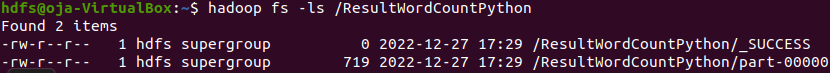
\includegraphics[width=\textwidth]{RauzatinurSyah/no8 wordcount python}
\caption{hasil langkah ke-8 }
\label{gam:hasil program WordCountPython}
\end{figure}

\begin{figure}[!ht]
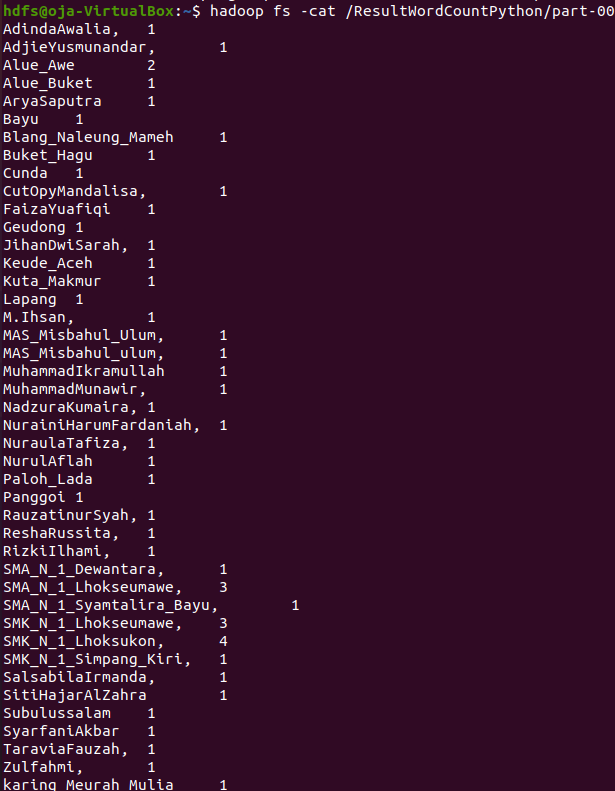
\includegraphics[width=\textwidth]{RauzatinurSyah/no9 wordcount python}
\caption{hasil langkah ke-9 }
\label{gam:hasil program WordCountPython}
\end{figure}

\end{enumerate}


\newday{\textbf{22 Desember 2022} - WordCount dengan pySpark}
\begin{enumerate}
\item Kendala dan Solusi
% jelaskan kendala dan penyebab yang dialami saat mengikuti praktikum serta solusi atau langkah-langkah yang telah dilakukan
\begin{itemize}

\item adapun kendalam pada praktikum ini terdapat pada langkah ke 6, yang dilakukan pengecekan hasil dengan printah "hadoop fs -ls /ResultWordCountPyspark" terdapat error yang menyatakan bahwa direktori tersebut tidak ada.

\item solusi yang diatasi pada kendala tersebut yaitu menulis kembali perintah "hadoop fs -ls /ResultWordCountPySpark" dengan "PySpark". perintah awal akan error dikarnakan direktori yang dibuat yaitu WOrdcountPySpark dengan kata spark diawali huruf kapital.
\end{itemize}

\item Kesimpulan\\
% berikan kesimpulan dari praktikum yang telah dikerjkan
adapun kesimpulan yang diperoleh yaitu program WordCount dengan PySpark berhasil dijalankan, dengan hasil screentshot sebagai berikut:

\begin{figure}[!ht]
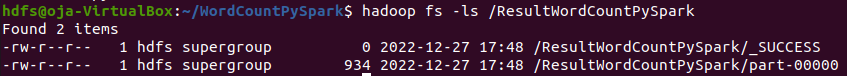
\includegraphics[width=\textwidth]{RauzatinurSyah/no6 wordcount Pyspark}
\caption{hasil langkah ke-6 }
\label{gam:hasil program WordCountPySpark}
\end{figure}

\begin{figure}[!ht]
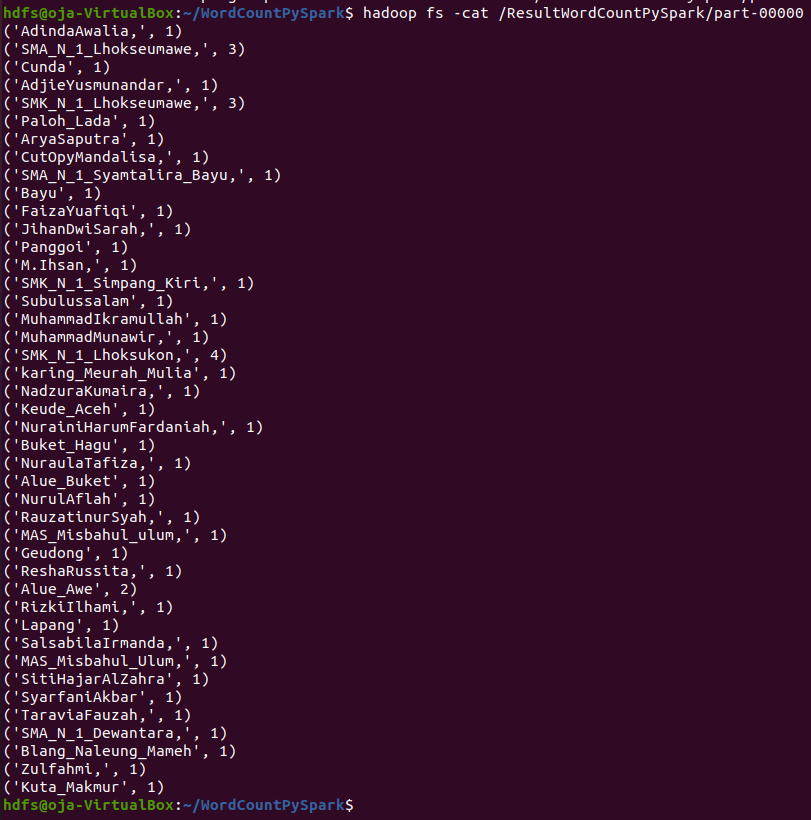
\includegraphics[width=\textwidth]{RauzatinurSyah/no7 wordcount Pyspark}
\caption{hasil langkah ke-7 }
\label{gam:hasil program WordCountPySpark}
\end{figure}
\end{enumerate}

\newday{\textbf{23 Desember 2022} - Tugas Individu}
\begin{enumerate}
\item Kendala dan Solusi
% jelaskan kendala dan penyebab yang dialami saat mengikuti praktikum serta solusi atau langkah-langkah yang telah dilakukan
\begin{itemize}
\item kendala yang terdapat pada tugas ini yaitu kesalah ketika menulis Kmeans pada sintak for dan kesalahan ketika menulis KMeans Assignments pada cluster assignment yang menyatakan bahwa KMeans Assignments tidak terdeskripsi
\item soslusi yang diberikan yaitu penulisan KMeans pada for ditulis dengan mengetab tombol tab pada keyboard 1 kali. adapun penulisannya adalah sebagai berikut

\newpage
\begin{figure}[!ht]
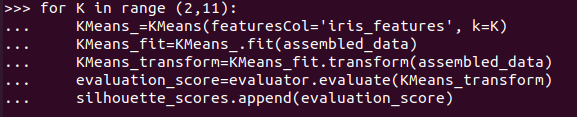
\includegraphics[width=\textwidth]{RauzatinurSyah/penulisan dalam for}
\caption{penulisan dalam for}
\label{gam:penulisan dalam for}
\end{figure}

dan untuk KMeans Assignemnt seharusnya tidak terdapat kesalah apabila langkah ke 6 tidak terloncati

\end{itemize}

\item Kesimpulan
% berikan kesimpulan dari praktikum yang telah dikerjkan

adapun kesimpulan pada tugas ini yaitu seluaruh program yang terdapat pada module dapat dijalankan dan mengahsilkan bebrapa table data dana figure. adapaun hasil yang diperoleh adalah sebagai berikut:

\begin{figure}[!ht]
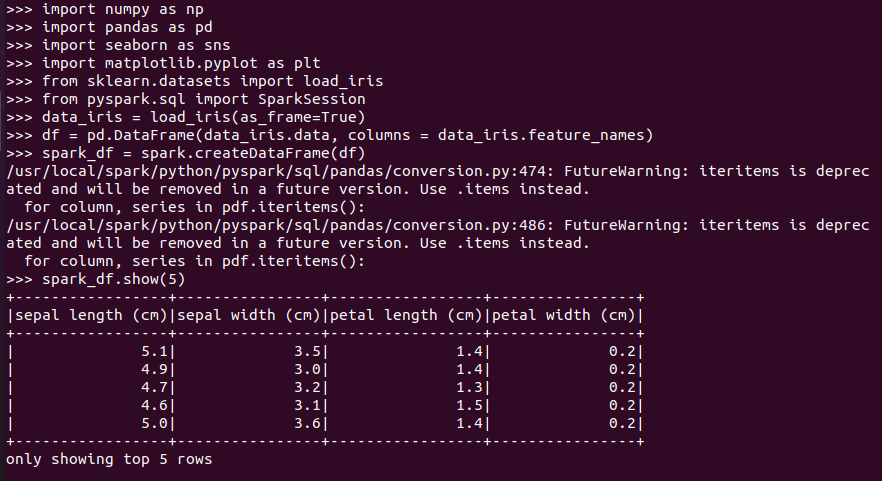
\includegraphics[width=\textwidth]{RauzatinurSyah/Tgs-individu no 3_4}
\caption{tampilan table 1}
\label{gam:hasil tugas individu}
\end{figure}

\begin{figure}[!ht]
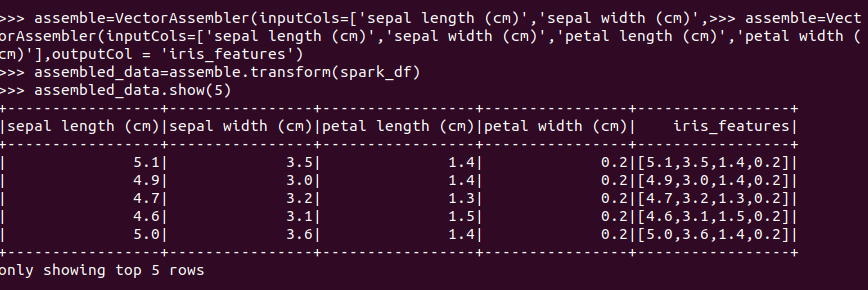
\includegraphics[width=\textwidth]{RauzatinurSyah/Tgs-individu no 5 assembled_datashow}
\caption{tampilan table 2}
\label{gam:hasil tugas individu}
\end{figure}

\begin{figure}[!ht]
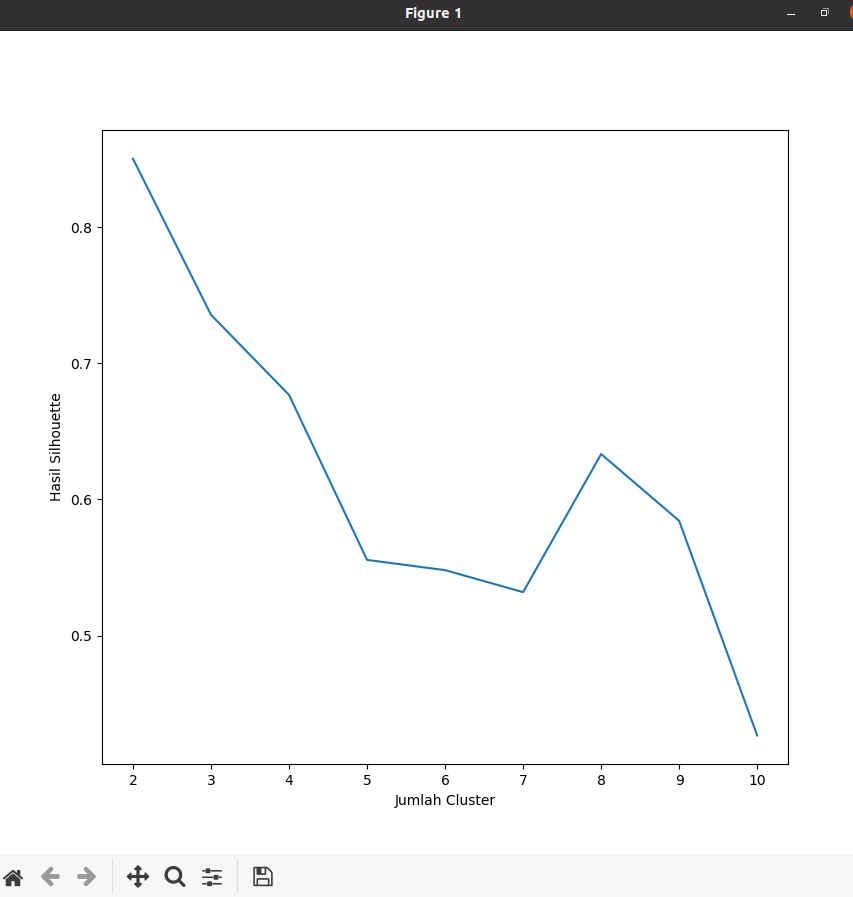
\includegraphics[width=\textwidth]{RauzatinurSyah/Tgs-individu no 5 figure}
\caption{tampilan figure 1}
\label{gam:hasil tugas individu}
\end{figure}

\begin{figure}[!ht]
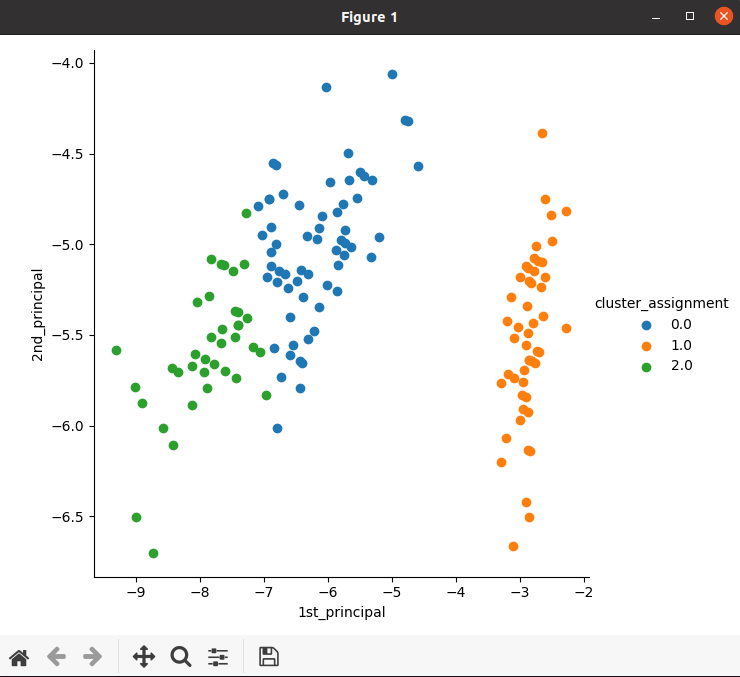
\includegraphics[width=\textwidth]{RauzatinurSyah/Tgs-individu no 6 figure}
\caption{tampilan figure 2}
\label{gam:hasil tugas individu}
\end{figure}

\end{enumerate}



